\documentclass{article}

% NeurIPS style (official neurips_2025.sty, in this folder). [preprint]: authors shown, no line numbers.
% It sets the page layout and loads natbib itself, so no geometry or natbib here.
\usepackage[preprint]{neurips_2025}
\usepackage[utf8]{inputenc}
\usepackage[T1]{fontenc}
\usepackage[colorlinks=false, urlcolor=magenta, citecolor=blue, pdfborder={0 0 0}]{hyperref}
\usepackage{url}
\usepackage{booktabs}
\usepackage{amsfonts}
\usepackage{nicefrac}
\usepackage{microtype}
\usepackage{xcolor}
\usepackage{graphicx}
\usepackage{amsmath}
\usepackage{amssymb}
\usepackage{paralist}
\usepackage{placeins}

\newcommand{\coderepo}{\url{https://github.com/Zhannyhong/bila}}

\title{Making Room on the Shelf: Closed-Loop Gap Creation and Learned Corrections for Robotic Book Reshelving\\[4pt]
\normalsize CS5478 Project}

\author{%
  Zhu Yu Hao\\ A0356892L \And Victor\\ A0258049W \And Zhan Hong\\ A0271539X
}

\begin{document}
\maketitle

\begin{abstract}
Prior work on robotic book placement assumes that the slot is already open, yet real shelves rarely leave a
gap for a returned book: its neighbours touch, lean into the space, or belong to a packed row. We study the
whole reshelving step in a MuJoCo simulation with real book models from the PBBM robot librarian and a
Franka Panda with a realistic wrist RGB-D camera. A closed-loop controller looks at the slot and chooses one
of four skills: stand up a leaning neighbour, widen the gap, shove a run of books into the row's free
space, or insert. With exact perception it places 97.5\% of books across 800 clear, tight, leaning and
packed rows, and 94.5\% of 200 rows of real books; with the camera and a learned spine segmenter it places
79\%. Scaling the camera's measured errors from zero to twice their size lowers success from 94.5\% to
49.5\% with the controller unchanged, so perception, not control, limits the system. Consistent with this,
neither a residual PPO policy for insertion nor a learned skill selector improves on the controller.
Code and instructions: \coderepo.
\end{abstract}

% =====================================================================================================
\section{Introduction}

Libraries have automated returns, sorting and shelf auditing, but putting a returned book back on the
shelf is still done by hand. Shelf-reading robots find misplaced books and report them to staff; they do
not move them. Prior work on robotic placement assumes the slot is open: the PBBM robot
librarian~\citep{sygo2023pbbm} places books against a shelf wall or at the end of a row, and residual-RL
book insertion~\citep{liu2026residual} assumes a gap wide enough to insert directly. Real shelves rarely
leave such a gap. We consider four row states: \textbf{clear} (the gap is wider than the book),
\textbf{tight} (narrower, but the neighbours can be pushed apart), \textbf{leaning} (a neighbour leans into
the slot) and \textbf{packed} (the neighbours touch, and room must be made by shoving a run of books along
the board).

We treat reshelving as a closed loop between perception and action: the robot looks at the slot, decides
whether the book fits, changes the row if it does not, inserts the book, and looks again. We ask (i)
whether a controller over a few gap-creation skills handles all four row states, (ii) how much a realistic
wrist camera costs and which of its errors matter, and (iii) whether learning, a residual PPO policy as
in~\citet{liu2026residual} or a learned skill selector, recovers the remaining failures. Our contributions:
\begin{compactenum}
  \item A MuJoCo~\citep{todorov2012mujoco} benchmark of randomized bookcases in the four row states, with the
        PBBM book models (sizes, masses, covers, hinged pages), a Franka Panda, a realistic wrist RGB-D camera,
        and an end-to-end book-return cart.
  \item A closed-loop controller over four skills (stand up, widen, shove, insert) that places 97.5\% of books
        across 800 rows with exact perception and 94.5\% of 200 rows of real books.
  \item An error-source analysis: success falls from 94.5\% to 49.5\% as the camera's measured errors are
        scaled from zero to twice their size, with the controller unchanged.
  \item An evaluation of a residual PPO policy and a fitted-Q skill selector on top of the controller,
        showing why neither helps, and a design finding for residual actions: corrections expressed as
        increments drift to their bounds, while target corrections do not.
\end{compactenum}

% =====================================================================================================
\section{Related Work}

\paragraph{Robotic librarians.} Library robots began with shelf auditing, reading RFID tags or spine labels
to report misplaced books. The PBBM robot librarian~\citep{sygo2023pbbm} is the most complete manipulation
system: a PR2 detects, segments and reads spines in a multi-stage perception pipeline, identifies each book
against a catalogue, and uses bimanual force-controlled skills to pull books out and place them. Placement
relies on an existing free location, and soft covers are a reported failure mode. We reuse its book models
and its reliance on force feedback, but make room for the book instead of assuming it, use a single arm
with a wrist camera, and evaluate over hundreds of randomized rows rather than a few trials.

\paragraph{Residual reinforcement learning for insertion.} Residual RL adds a learned correction to a
hand-designed controller, so learning starts from competent behaviour~\citep{johannink2019residual,
silver2018residual}. \citet{liu2026residual} apply it to book insertion: a nominal controller aligns the
book with the slot, and PPO adds bounded incremental corrections to position, yaw and pitch from a 12-D
geometric state and learns when to release. It raises success from 27\% to 93\% in simulation and to 63\%
on hardware, with gains largest where the nominal controller is weakest and none below 2\,mm of
clearance. We follow its design (PPO, bounded task-space corrections, a progress reward) but our nominal
controller already succeeds on most insertions, our residual sees the camera's estimate rather than true
geometry, and the neighbouring books are free bodies the insertion can push.

\paragraph{Skill selection and offline RL.} Choosing among parameterized skills makes long-horizon
manipulation learnable~\citep{dalal2021raps, nasiriany2022maple}. When episodes are expensive the
selector can be learned offline from logged episodes by fitted Q iteration~\citep{ernst2005fqi,
riedmiller2005nfq}, which we use to choose the controller's next skill.

\paragraph{Shelf perception.} Instance segmentation~\citep{he2017maskrcnn} separates books in an image, and
spine text identifies them. Insertion needs more: metric geometry at the millimetre level. We fit spines in
3D from depth and correct the camera pose with fiducial markers~\citep{garrido2014aruco}.

% =====================================================================================================
\section{Method}

Figure~\ref{fig:pipeline} summarises the system. Perception turns wrist RGB-D images into a shelf estimate
$\hat{s}$; a skill selector (rules, or a learned policy) maps $\hat{s}$ to the next skill; each skill is a
sequence of planned Cartesian moves, some of them contact moves; during the insertion's contact moves a
residual policy may correct the hand's target. After every skill the robot looks again.

\begin{figure}[t]
\centering
\scriptsize
\begin{verbatim}
 RGB-D views --> perception --> s_hat --> skill selector --> skill --> planned moves --> arm
                                  ^                            |          ^ (contact moves)
                                  |                            |          +-- residual pi(o_t) <-- s_hat, q, wrist F/T
                                  +-------- look again <-------+
\end{verbatim}
\caption{The closed loop. The robot re-observes the row after every skill.}
\label{fig:pipeline}
\end{figure}

\subsection{Simulation}

\paragraph{Scene.} A bookcase of 3--5 levels with randomized width, depth and board heights. The target row
holds free-standing books, placed and then settled by physics so leaning and touching books are in real
resting poses. The books are the PBBM catalogue's~\citep{sygo2023pbbm}: each keeps its size, mass and
textured cover, and its pages are cut into four sections hinged at the spine so it can splay when pushed.
A scenario sets the row's initial state, and a seed sets everything random (layout, books, friction,
camera noise), so disjoint seed ranges give disjoint scenes. Frames: $x$ along the row, $y$ out of the
shelf, $z$ up.

\paragraph{Robot and success.} A Franka Panda~\citep{menagerie2022} on a lift that tracks the target level,
with fingers replaced by bars 10\,mm wide and 12\,cm long so they fit between books, a force/torque
sensor at the flange and an RGB-D camera (modelled on the RealSense D405) on the wrist. Any arm contact
with the shelf over 1\,N counts as a collision. The book is \emph{placed} if it ends upright, in place (its
spine within 10\,mm of the more protruding neighbour's) and released.

\subsection{Perception from a wrist camera}

Before touching the row the arm takes three RGB-D views along it, and it looks again after every skill
that moves books. A Mask R-CNN~\citep{he2017maskrcnn} (ResNet-50 FPN, fine-tuned on 2{,}938 simulated images)
segments the spines; on 309 held-out images it finds 93\% of visible target-row books with mean IoU 0.93.
Inside each mask, depth pixels are back-projected and a planar rectangle is fitted robustly to the spine
face, giving each book's position, thickness $t_i$, height, lean and swivel. From these the estimate
derives the gap width at eight heights and the free space on each side of the row,
$r_\pm = L_\pm - \sum_{i \in \pm} t_i$, with $L_\pm$ the length of that side.

\paragraph{Camera errors and fiducial correction.} Depth follows the D405: noise growing with depth, edge
spread and a small offset. The camera's mounting has a calibration error drawn per episode (about
1.5\,mm and $0.3^\circ$ per axis), which shifts the whole estimate by up to 11\,mm (95th percentile); the edge
spread makes every book appear 2.4--3.8\,mm too thick. ArUco markers~\citep{garrido2014aruco} with known
positions every 15\,cm along each board's front edge give the camera pose relative to the shelf in each
image. Only the along-row and vertical components are corrected; a full 6-DoF PnP correction is poorly
conditioned in depth at this distance and moved the estimate by 3--19\,mm.

\subsection{Closed-loop controller over gap-creation skills}

With the estimated leans $\lambda_\pm$ of the slot's neighbours, the gap $g$, the book's thickness $t$ and a
margin $m = 6$\,mm, the controller takes
\begin{equation}
\text{skill}(\hat{s}) =
\begin{cases}
\texttt{stand\_up}(\pm) & \text{if } \lambda_\pm > 5^\circ \text{ into the slot},\\
\texttt{widen} & \text{else if } g < t + m \text{ and the stacked fingers fit in the gap},\\
\texttt{shove} & \text{else if } g < t + m,\\
\texttt{insert} & \text{otherwise,}
\end{cases}
\end{equation}
retrying a skill that falls short up to a cap. \emph{Stand up} lifts a leaning neighbour along an arc about
its pivot corner, or pinches it near the spine and swings it up. \emph{Widen} puts the stacked fingers into
the gap and pushes one neighbour aside until the gap is $t + m$. \emph{Shove} pushes the books beside a
touching neighbour back so it stands proud, pinches it, and shoves it and every book beyond it into the
free space $r_\pm$. \emph{Insert} rests the book on the board and slides it in until the wrist force rises
by 35\,N, releases it, and pushes the spine home, stopping at 40\,N. Each skill ends with the hand out of
the shelf, so skills compose in any order. Joint moves are collision-checked; Cartesian paths use damped
least-squares IK.

\subsection{Residual PPO for insertion}

During the insertion's two contact moves (slide and push) a policy $\pi_\theta$ corrects the hand's target at
25\,Hz. The actor sees $o_t \in \mathbb{R}^{155}$, only quantities a real robot has: the shelf estimate
around the slot, joint states, the hand pose, the change in wrist force and torque, and the controller's
phase, target and correction so far. The critic also receives privileged state~\citep{pinto2018asymmetric}
(true book poses, masses, friction, grasp error, contact forces).

\paragraph{Action as a target correction.} The action $a_t \in [-1, 1]^5$ ($x, y, z$, yaw, pitch) is mapped onto
per-phase bounds $[\ell, u]$ ($\pm 4$\,mm sideways, $-8$ to $+2$\,mm in depth, $\pm 1.5^\circ$):
\begin{equation}
c^\ast_t = \max(a_t, 0) \odot u + \min(a_t, 0) \odot (-\ell), \qquad
c_t = \Pi_{[\ell,u]}\!\left(c_{t-1} + \operatorname{clip}(c^\ast_t - c_{t-1}, -\delta, \delta)\right),
\end{equation}
with rate limit $\delta = (3\,\text{mm}, 3\,\text{mm}, 3\,\text{mm}, 0.4^\circ, 0.4^\circ)$. The hand tracks the
controller's pose offset by $c_t$; with the last layer initialised to zero, the untrained policy \emph{is}
the controller. In the incremental form of~\citet{liu2026residual}, $c_t = c_{t-1} + a_t \odot \delta$, any
mean action $\bar a$ makes the correction grow linearly, $\|c_t\| \approx t\,|\bar a|\,\delta$: over a slide of
120--170 decisions a mean action of 0.1 drifts 6\,mm, more than a book's 5--7\,mm of clearance, whereas the
target form holds 0.4\,mm. A fixed policy outputting 0.1 places 3 of 8 books with increments and 8 of 8 with
targets.

\paragraph{Reward and training.} The reward pays $+1$ per cm of progress towards an accepted placement and
$-0.5$ per cm the other books move, penalises wrist force above 60\,N, action changes and time, and ends
with $+10$ (placed), $-5$ (inserted, not placed) or $-10$ (jammed or collided); Appendix~\ref{app:details}
gives the formula. Actor and critic are two-layer MLPs (256 units) trained with
PPO~\citep{schulman2017ppo}. Each episode draws a new scene, calibration error, depth noise and grasp
error, on the rendered camera with learned masks. Because the controller fails only a few percent of
insertions, training pools are balanced 50/50 between its failures and successes, split by layout.

\subsection{Learned skill selection and the book-return cart}

A learned selector replaces the rules' fixed order and retry caps, choosing among eight actions (the four
skills with both stand-up sides, a wider widening, setting a jammed book aside, and giving up) from a
15-feature state, with a mask that admits only feasible actions. $Q$ is learned offline by fitted Q
iteration from logged episodes of the rules with random deviations (Appendix~\ref{app:details}).

To test the pieces end to end, the Panda is mounted on a lift on a book-return cart (Figure~\ref{fig:cart}).
It reads the call-number stickers of the books in its tray, looks each up in a shelf map (each row's height
and call-number range), lifts to the row, reads the row's stickers to find the slot, makes room, and
picks the book from the tray to insert it. The book is held only by friction under the gripper's 70\,N
squeeze (the Franka Hand's continuous rating; 61--70\,N measured per side). The robot uses only the tray's
layout, the shelf's depth and the books' catalogue sizes: it assumes the book stays where the hand closed
on it and is not told how it shifts in the grip.

\begin{figure}[t]
\centering
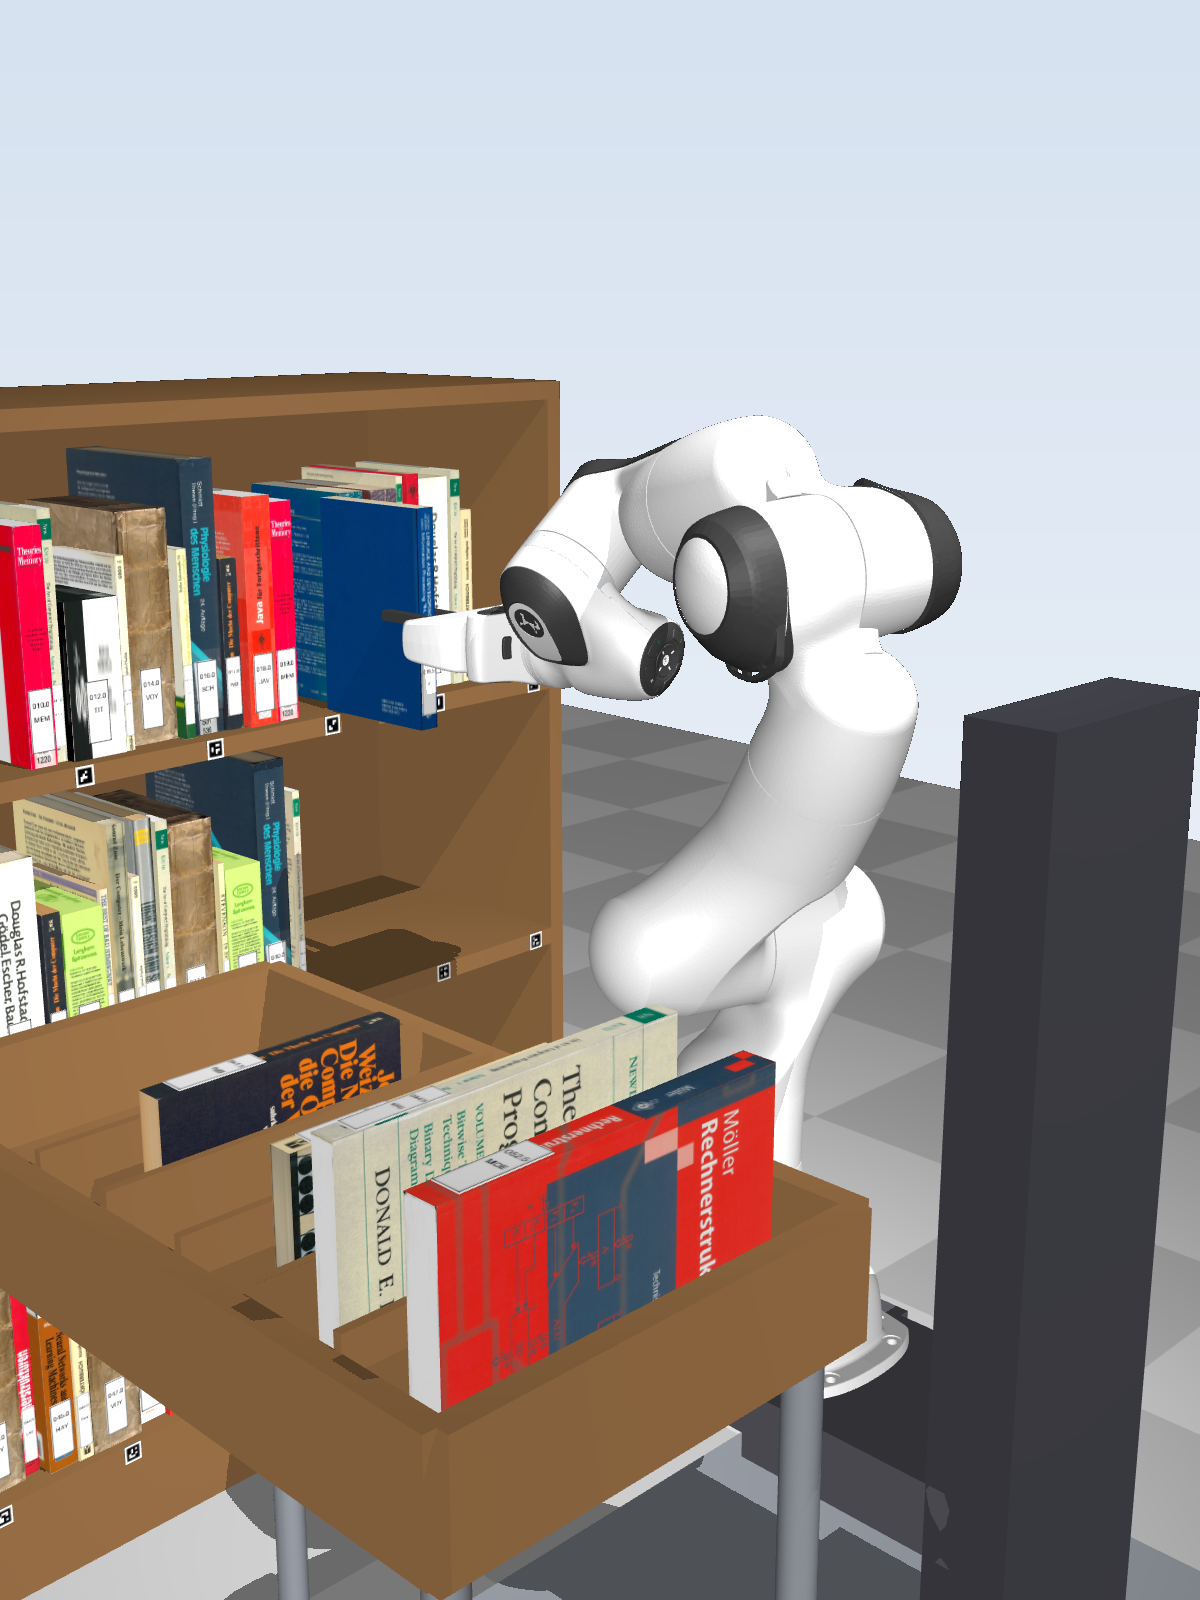
\includegraphics[width=0.36\linewidth]{figures/cart.png}
\caption{The book-return cart: a Franka Panda on a lift, a tray of returned books with call-number
stickers, and a bookcase of PBBM books with ArUco markers on the boards' front edges.}
\label{fig:cart}
\end{figure}

% =====================================================================================================
\section{Experiments}

\paragraph{Setup.} We evaluate on 200 rows per scenario with box-shaped books, and on 50 rows per scenario
(seeds 0--49) with the real PBBM books. Perception is either \emph{truth} (the simulator's book poses),
\emph{camera} (the rendered wrist camera with D405 noise and a per-episode calibration error, with the
simulator's or the learned masks, with or without fiducial correction), or \emph{noisy} (the true shelf plus
errors drawn from the learned-mask camera's measured error distribution, scaled by a factor; no
rendering). Nothing learned was trained or tuned on its test rows. Conditions are compared on the same
rows with the exact McNemar test on the rows only one of them places.

\subsection{The controller across row states}

\begin{table}[t]
\centering
\caption{Books placed. Box books: 200 rows per scenario, camera with the simulator's masks, no fiducial
correction. Real books: 50 rows per scenario, four page sections, learned segmenter.}
\label{tab:main}
\begin{tabular}{llccccc}
\toprule
 & Perception & Clear & Tight & Leaning & Packed & All \\
\midrule
Box books  & Truth  & 200 & 197 & 199 & 184 & 97.5\% \\
           & Camera & 189 & 139 & 188 &  94 & 76.3\% \\
\midrule
Real books & Truth                        & 50 & 50 & 48 & 41 & 94.5\% \\
           & Camera + fiducial correction & 47 & 41 & 44 & 26 & 79.0\% \\
           & Camera, no correction        & 47 & 38 & 45 & 25 & 77.5\% \\
\bottomrule
\end{tabular}
\end{table}

With exact perception the controller solves nearly every clear, tight and leaning row and 82--92\% of packed
rows (Table~\ref{tab:main}), row states in which prior systems~\citep{sygo2023pbbm, liu2026residual} would not
start. Real books with hinged pages change little. Neighbours move a few millimetres, except in packed
rows, where the shove moves a run of books by design (median 59\,mm). Most remaining failures are packed
rows in which no collision-free arm configuration reaches the slot.

The camera costs 16 points on real books: 33 rows are placed only with exact perception and 2 only with the
camera ($p = 4 \times 10^{-8}$). The losses concentrate in packed rows (82\%\,$\to$\,52\%) and tight rows
(100\%\,$\to$\,82\%). In packed rows the cause is systematic: every book appears 2.4--3.8\,mm too thick, so along
a side of 10--15 books the free space is underestimated by 30--60\,mm and the controller declines a shove
that would have worked. In tight rows, pushes go to faces the camera placed a few millimetres off, and books
catch a neighbour on the way in. The camera also takes 2--4 times longer, mostly spent looking.

\subsection{Where the errors come from}

\paragraph{Fiducial correction.} With box books and the simulator's masks, correcting the camera pose raises
tight-row success from 67\% to 87\% and clear rows from 95\% to 97\% (100 rows each; $p = 3 \times 10^{-5}$). With
real books and the learned segmenter it does not help significantly (158 against 155 rows; $p = 0.58$): the
learned masks' own errors, which a pose correction cannot remove, take a larger share of the error.

\paragraph{Error-source sweep.} If the camera's errors decide the outcome, success should fall as they grow
while the controller and rows stay the same. Table~\ref{tab:sweep} adds the camera's measured errors to exact
perception, scaled from 0 to 2. Success falls steadily, each step is significant on paired rows
($p < 10^{-5}$), and the fall is steepest in tight and packed rows. Since only the perception error changes,
the losses come from what the robot believes about the row, not from how it acts on it. The error model
is pessimistic: the rendered camera (79\%) matches it at about half its scale (80.5\%; $p = 0.71$), not at full
scale (70\%; $p = 0.008$).

\begin{table}[t]
\centering
\caption{Real books placed out of 50 rows per scenario with exact perception plus the camera's measured
errors scaled by $k$. The controller and rows are the same in every row of the table.}
\label{tab:sweep}
\begin{tabular}{lccccc}
\toprule
$k$ & Clear & Tight & Leaning & Packed & All \\
\midrule
0 (truth) & 50 & 50 & 48 & 41 & 94.5\% \\
0.5       & 49 & 40 & 49 & 23 & 80.5\% \\
1         & 46 & 31 & 45 & 18 & 70.0\% \\
2         & 37 & 22 & 31 &  9 & 49.5\% \\
\bottomrule
\end{tabular}
\end{table}

\subsection{Learned components}

\paragraph{Residual PPO.} Under the training conditions the controller fails only 2--6\% of the insertions
it reaches (6 of 250 in clear rows, 11 of 241 in tight, 16 of 247 in leaning). On 20 validation cases
balanced between failures and successes, the best checkpoint rescues 2 of the controller's 10 failures and
loses none (12/20 against 10/20, $p = 0.5$), optimistic since these cases also selected it. On a held-out pool
of 24 cases from unseen layouts (the controller's 12 failures among 355 labelled cases plus 12 successes),
the controller places 15 and the residual places 15, rescuing one and losing one. The residual acts only
during insertion, so it cannot fix an underestimated free space or a gap left too narrow, which is where
the camera's losses occur. This is the main difference from~\citet{liu2026residual}, whose nominal
controller fails 73\% of insertions.

\paragraph{Learned skill selection.} On 25 rows per scenario with the noisy perception model, the learned
selector ties the rules at 76 of 100 rows ($p = 1$). It chooses differently on about half the rows, but its
wins and losses cancel: it shoves before standing up when a leaning book is wedged and gives up less often,
but it learned to skip some stand-ups, leaving a leaning book that later catches the inserted one.

\paragraph{End-to-end cart.} The full cart pipeline places 10 of 12 scenes (three seeds per scenario), with
the rules and the learned selector alike; both failures are packed scenes where the arm cannot reach the
slot. Without privileged grasp information, the robot's belief about the held book is 1.6--3.5\,mm and
0.3--0.7$^\circ$ off at release, and the result is the same 10 of 12 as when it was given the book's true pose,
so the insertion tolerates a few millimetres of in-hand error. Recordings are in the repository
(\texttt{runs/cart\_demo\_*.mp4}).

% =====================================================================================================
\section{Conclusion}

We studied robotic reshelving including the step prior work assumes away: making room for the book. A
closed-loop controller over four gap-creation skills places 97.5\% of books across clear, tight, leaning and
packed rows with exact perception, and 79\% of real-book rows from a wrist RGB-D camera with learned
segmentation. Success follows the size of the perception error, from 94.5\% without it to 49.5\% at twice its
measured size, and the errors that matter are systematic (a thickness bias summed along the row, a
calibration shift) rather than random. Neither an insertion residual nor a different choice of skill can
correct a wrong belief about the row, so both learned layers had little to fix: the reverse of
\citet{liu2026residual}, where a weak nominal controller leaves most of the gain to learning.

\paragraph{Limitations.} Everything is in simulation, and \citet{liu2026residual} report a drop from 98.5\% to
63.3\% on hardware. Books are rigid apart from their hinged pages, so soft covers, a failure mode reported
by~\citet{sygo2023pbbm}, are not modelled. The grasp's friction is not calibrated: the pads' sliding friction
(1.0) suits rubber pads on matte covers, and their torsional friction is 3--5 times what a 10\,mm pad gives,
so heavy books twist less in the grip than on hardware. Test sets for the learned layers are small (20
validation and 24 held-out residual cases, 12 cart scenes).

\paragraph{Future work.} The largest loss is the camera's thickness bias, which a calibrated edge-spread
correction or the catalogue's known thicknesses would remove directly. Feeling the neighbours' faces with
the fingertips before pushing, and learning residuals for the gap-creation skills (widen, shove) rather
than for insertion, would act where most failures occur.

\bibliographystyle{unsrtnat}
\bibliography{references}

% =====================================================================================================
\appendix

\section{Code and reproduction}
\label{app:code}

The code is at \coderepo; its README describes the simulator, every component and the experiments in
detail. Setup and the main commands (run from the repository root):
\begin{verbatim}
git clone --recurse-submodules https://github.com/Zhannyhong/bila && cd bila
uv sync                                 # add --group rl for the segmenter and PPO (torch)

# watch the book-return cart (macOS: mjpython; elsewhere: python)
uv run mjpython -m bila.control.cart_demo --scenario tight --view
uv run python -m bila.viz.live_view --scenario tight        # web page: wrist and scene cameras

# the controller on one row: clear | tight | leaning | packed
uv run python -m bila.control.insert_book --scenario tight --seed 0

# Table 1, real books, 50 rows per scenario (perception: truth | camera | noisy-learned)
uv run python -m bila.control.eval_reshelve run --perception truth --catalogue --book-pages 4 \
    --book-meshes --scenarios clear tight leaning packed --seeds 0:50 --out results/truth.jsonl
\end{verbatim}
The scripts behind every table are in \texttt{results/paper/run.sh}, and
\texttt{notebooks/08\_paper\_draft.ipynb} recomputes the tables from the result files.

\section{Additional details}
\label{app:details}

\paragraph{Residual reward.} With $d_t$ the book's distance from an accepted placement (m), $D_t$ the summed
displacement of the other books (m), $F_t$ the peak wrist force (N) and $\Delta_t$ the change of correction,
\begin{equation*}
r_t = 100\,(d_{t-1} - d_t) - 50\,(D_t - D_{t-1}) - 0.01\,[F_t - 60]_+ - 0.1\,\|\Delta_t / \delta\|^2 - 0.01
+ \mathbb{1}_{\text{end}} \cdot \{+10,\ -5,\ -10\}.
\end{equation*}
PPO uses a clipped surrogate with $\epsilon = 0.2$, $\gamma = 0.99$, GAE $\lambda = 0.95$, and an action scale
ramped from 0.25 to 1 over the first 50k decisions.

\paragraph{Skill selector.} The actions are \texttt{insert}, \texttt{widen}, \texttt{widen\_more} (to $t +
10$\,mm), \texttt{shove}, \texttt{stand\_up\_left}, \texttt{stand\_up\_right}, \texttt{set\_aside} (back a
jammed book out and look again) and \texttt{give\_up}. The 15 state features are the neighbours' leans, the
gap's spare width against $t$ and $t + m$, the room for the fingers, the free space on each side, $t$, the
counts of each skill taken, jams, steps, whether the last skill achieved anything, and whether a book is
held. The reward is $-0.02$ per step and $+1$ for a placed book; $Q$ is an MLP (15--64--64--8) refitted for 8
rounds of fitted Q iteration on episodes from seeds 5{,}000--5{,}059, and tested on seeds 0--24.

\end{document}
